\section{Results and Discussion}

\subsection{Boundary Detection}

\begin{table}[t]
\caption{Boundary detection results (frozen weights, $\beta{=}0$) on 20 TIMIT test utterances, averaged over 10 random seeds. Prominence threshold is oracle-selected per utterance (Section~\ref{sec:eval}).}
\label{tab:boundary}
\centering
\small
\begin{tabular}{@{}lccc@{}}
\toprule
 & \textbf{Precision} & \textbf{Recall} & \textbf{F1} \\
\midrule
Level~1 (phone) & 0.67 & 0.74 & \textbf{0.69} \\
Level~2 (word) & 0.51 & 0.80 & \textbf{0.61} \\
\midrule
L1-direct (word baseline) & 0.27 & 0.94 & 0.42 \\
\bottomrule
\end{tabular}
\vspace{-10pt}
\end{table}

The Level~1 area achieves a phone boundary F1 score of 0.69, while the hierarchical Level~2 area achieves a word boundary F1 score of 0.61. This improves substantially over using the Level~1 change signal directly at the word level (F1$=$0.42), a gain of $+$0.19 (Table\ref{tab:boundary}). This demonstrates the effectiveness of the proposed framework for boundary detection across different timescales. Optimisation reveals two main trends. First, using a coarser temporal resolution and fewer mel bins reduces variability within phones, which in turn lowers false boundary detections. Second, Level~1 and Level~2 operate on different timescales: Level1 needs a very high refractory rate ($\rho{=}0.989$) to strongly suppress rapid re-firing, whereas Level2 uses a much lower refractory rate ($\rho{=}0.092$) and a larger minimum peak distance ($d{=}7$ vs.\ 3 frames) to reflect the longer duration of words.


\subsection{Classification}

\begin{table}[t]
\caption{Classification results with per-class RecurrentAreas trained using ABS plasticity (Eq.~\ref{eq:abs}) and scored by trajectory resonance (Eq.~\ref{eq:resonance}).}
\vspace{-10pt}
\label{tab:classification}
\centering
\small
\begin{tabular}{@{}lcc@{}}
\toprule
 & \textbf{Phone} & \textbf{Word} \\
 & (TIMIT) & (Speech Cmds) \\
\midrule
Classes $C$ & 39 & 10 \\
Chance accuracy & 2.6\% & 10.0\% \\
Test samples & 4{,}328 & 2{,}000 \\
\midrule
MFCCs $M$ & 11 & 19 \\
Pop.\ neurons $N_\mathrm{pop}$ & 14 & 9 \\
Input dim.\ $n_\mathrm{input}$ & 154 & 171 \\
Area size $n$ & 2{,}250 & 4{,}655 \\
Cap $k$ (\% sparsity) & 732 (32.5\%) & 815 (17.5\%) \\
Learning rate $\beta$ & $3.1{\times}10^{-4}$ & $3.6{\times}10^{-3}$ \\
Epochs & 13 & 2 \\
\midrule
\textbf{Accuracy} & \textbf{47.5\%} & \textbf{45.1\%} \\
\bottomrule
\end{tabular}
\vspace{-10pt}
\end{table}

Using per-class RecurrentAreas trained on population-coded MFCCs (Section~\ref{sec:traj_scoring}), we evaluate classification on both TIMIT phones and Google Speech Commands words (Table~\ref{tab:classification}).

On TIMIT, the system classifies ground-truth-bounded segments across 39 phone classes, achieving \textbf{47.5\%} accuracy (chance 2.6\%). On Google Speech Commands, it classifies whole-word utterances across 10 classes, achieving \textbf{45.1\%} accuracy (chance 10.0\%). Both tasks use ABS plasticity (Eq.~\eqref{eq:abs}) and resonance scoring. As shown in Figure~\ref{fig:phoneme_cm}, confusions predominantly follow phonetic similarity: fricatives cluster (\textit{s}$\leftrightarrow$\textit{sh}$\leftrightarrow$\textit{th}$\leftrightarrow$\textit{z}), low vowels cluster (\textit{aa}$\leftrightarrow$\textit{ah}$\leftrightarrow$\textit{aw}$\leftrightarrow$\textit{ay}), and nasals cluster (\textit{m}$\leftrightarrow$\textit{n}$\leftrightarrow$\textit{ng}). The system discriminates well between broad phonetic categories (vowels vs.\ fricatives vs.\ nasals) but struggles within categories where spectral envelopes overlap. This suggests that the population-coded MFCC representation preserves phonetic similarity structure and the per-class recurrent dynamics capture category-level spectral signatures well but struggle with fine intra-category distinctions. Stops (\textit{b}, \textit{d}, \textit{g}, \textit{k}, \textit{p}) remain the most challenging, possibly because their brief, transient spectra provide insufficient frames for the trajectory scoring to accumulate a discriminative signal.

\begin{figure}[t]
    \centering
    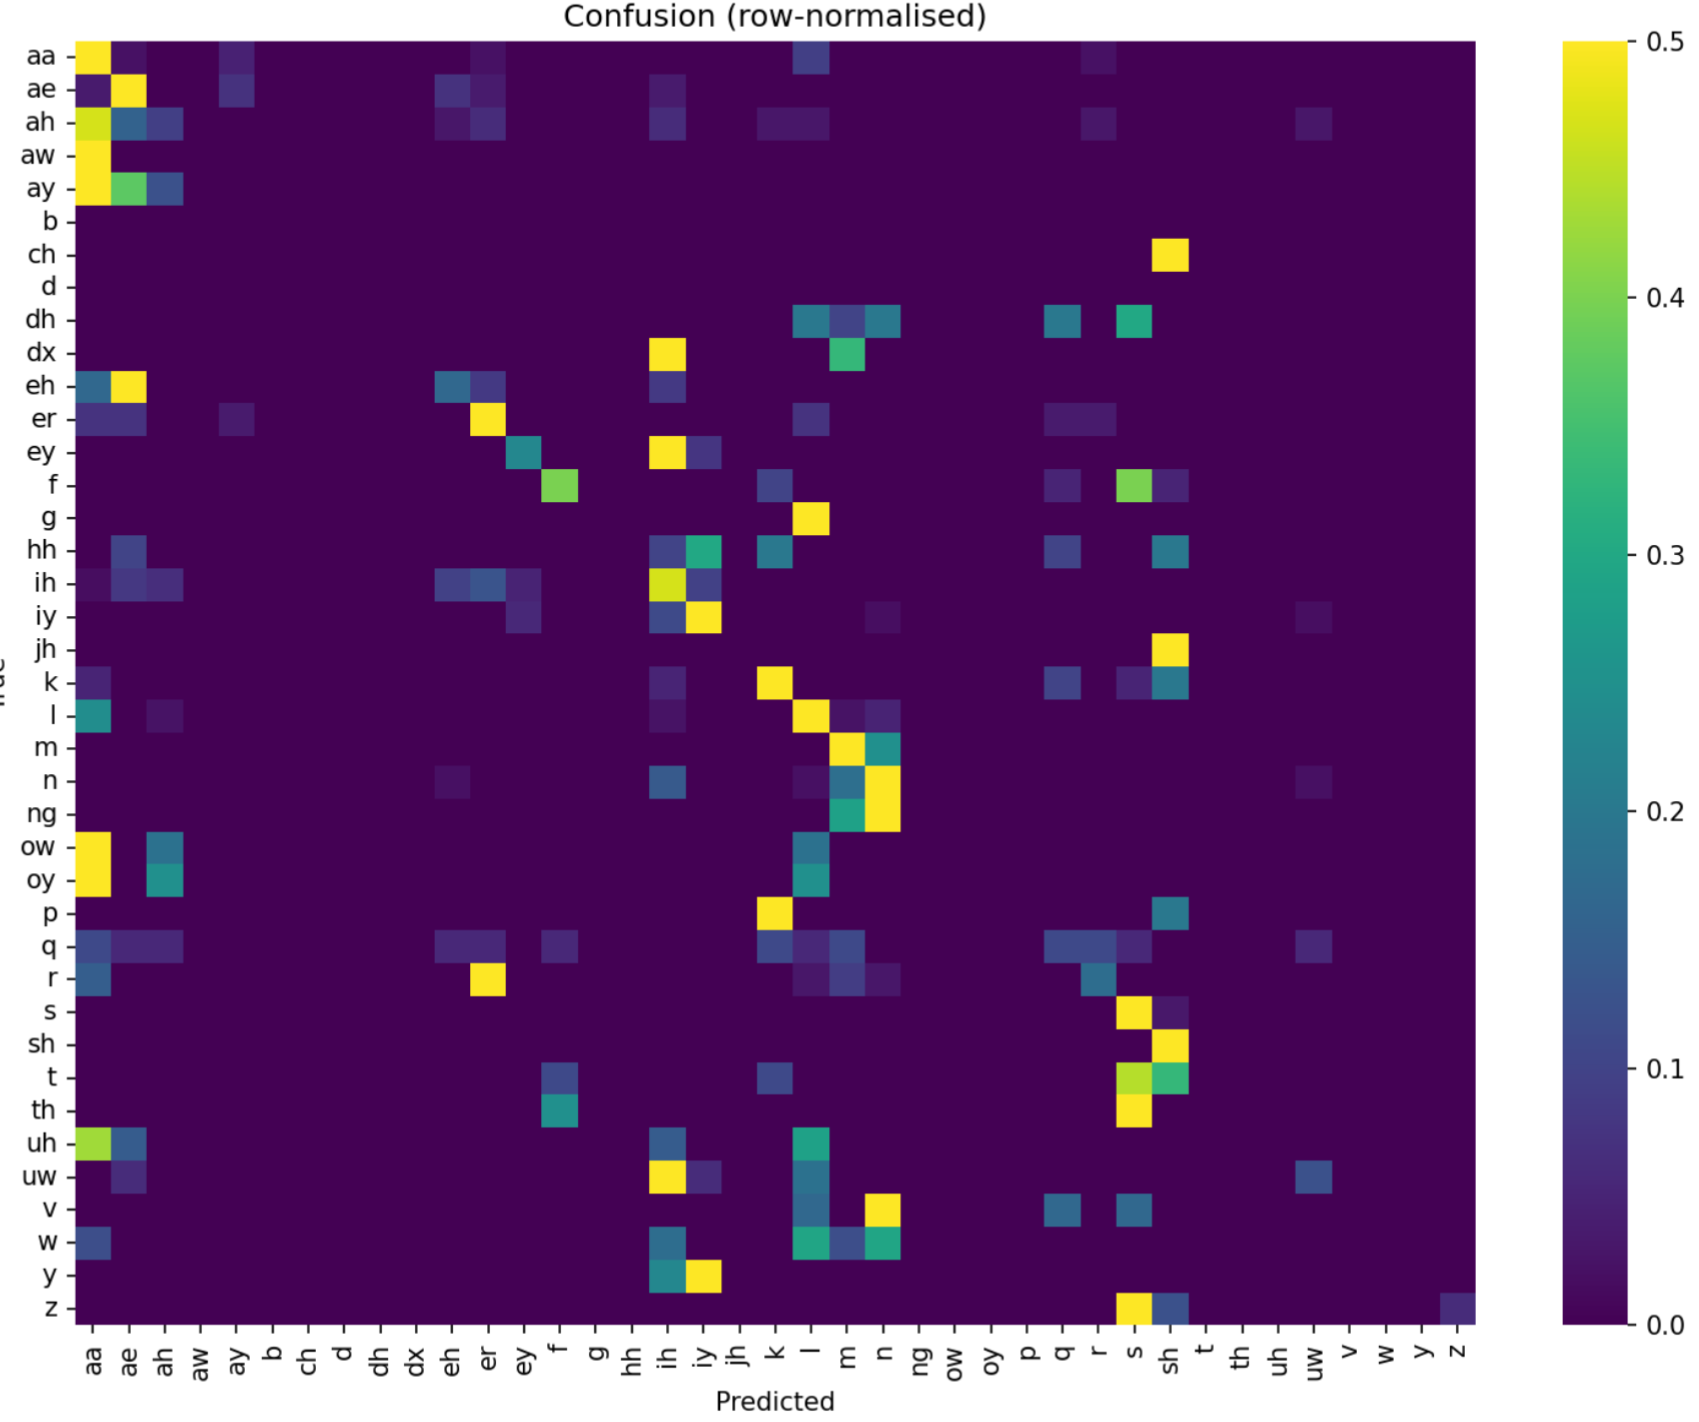
\includegraphics[width=0.8\columnwidth]{figures/phoneme_confusion_matrix.png}
    \vspace{-10pt}
    \caption{Row-normalised confusion matrix for phone classification on TIMIT (39 classes). Confusions follow phonetic similarity: fricatives (\textit{s}, \textit{sh}, \textit{th}, \textit{z}), low vowels (\textit{aa}, \textit{ah}, \textit{aw}), and nasals (\textit{m}, \textit{n}, \textit{ng}) form visible off-diagonal clusters.}
    \vspace{-10pt}
    \label{fig:phoneme_cm}
\end{figure}


\subsection{Discussion}

These results demonstrate that refractory adaptation in sparse assembly areas can serve as an unsupervised temporal boundary detector for speech. The key insight is that refractory suppression converts temporal change in the input into spatial change in the assembly: when the spectral content shifts (e.g.\ at a phone boundary), previously-active neurons are suppressed, forcing recruitment of a different assembly. The magnitude of this spatial change, measured by assembly overlap, provides a continuous boundary signal without any training. 

The hierarchical application of this mechanism mirrors the temporal hierarchy of speech: phone boundaries occur every 50--100\,ms, while word boundaries occur every 200--500\,ms. By cascading two refractory areas with different dynamics, the system naturally separates these timescales. 

For classification, per-class assembly areas enable the system to learn class-specific spectro-temporal trajectories. Each area operates as an independent dynamical system with its own attractor landscape shaped by Hebbian plasticity. A correctly matched area produces constructive interference between its learned dynamics and the input trajectory, while mismatched areas produce destructive interference as the input conflicts with the stored attractor structure. This is fundamentally different from deep learning, where classification is a static mapping from a final hidden state; here, the temporal dynamics \textit{are} the representation. The recurrent connections implicitly capture spectral dynamics (analogous to delta features in classical ASR~\cite{Rabiner89-ATO}) without explicitly computing derivatives; the recurrence \textit{is} the temporal derivative.

Interestingly, the two tasks favour different input representations: boundary detection works best with probabilistically binarised mel spectrograms, while classification works best with population-coded MFCCs. This suggests the representations capture complementary aspects of the signal: mel spectrograms preserve the fine temporal change structure needed for boundary detection, while MFCCs provide the pitch-invariant spectral identity needed for class discrimination.

\section{Conclusion}
The proposed AC-based dynamical system demonstrates that sparse assembly dynamics can effectively address two core speech tasks, unsupervised segmentation and supervised phone classification, directly from continuous audio, without backpropagation or the need to learn dense representations. By integrating probabilistic neural encodings, the hierarchical refractory areas, and trajectory-based classification, the framework employs simple local plasticity rules to learn stable assemblies that both detect boundaries and discriminate categories. Results on standard speech benchmarks show that recurrent, sparse assembly dynamics are promising in low-data settings, while offering a biologically grounded alternative to conventional deep learning approaches.

There are several limitations to our approach. First, the per utterance oracle prominence selection used for boundary detection provides an upper bound (Section~\ref{sec:eval}); using a globally fixed threshold reduces F1 by approximately 0.05--0.10. Second, classification relies on supervised labels to train the per class areas. A fully unsupervised system would require discovering phones categories directly from continuous speech, likely demanding richer and more structured multimodal assembly representations. Developing such mechanisms within AC frameworks for speech remains an important direction for future work. Third, although classification accuracy is well above chance on both tasks (Table~\ref{tab:classification}), it still not as accurate as established deep learning baselines. More expressive input representations or moderately more complex architectures may further improve performance.


Despite these limitations, AC based models hold tremendous promise for the future. Treating speech and audio as trajectories in a dynamical system allows, in principle, unbounded temporal context encoded in the evolving neural state, whereas transformer architectures are constrained by a fixed context window and incur quadratic computational cost with respect to sequence length. To solve a harder problem or take into account a longer context, deep learning systems need to be made bigger. AC based systems allow for the possibility that they just need more time.




